\documentclass[12pt,a4paper]{../krautsourcing/homework}
\usepackage[utf8]{inputenc}
\usepackage[ngerman]{babel}
\usepackage[T1]{fontenc}
\usepackage{amsmath}
\usepackage{graphicx}
\usepackage{amsfonts}
\usepackage{amssymb}
\usepackage{lmodern}
\usepackage{amsmath}
\usepackage{amssymb}
\usepackage{paralist}
\usepackage{tabularx}
\usepackage{tikz}
\usepackage{mathtools}
\usetikzlibrary{automata,positioning,petri,calc,backgrounds}

\author{Ruben Felgenhauer,\\Alexander Hildebrandt,\\Leonhard Reichenbach}
\datef{06}{12}{2015}
%\date{\today}
\course{Formale Grundlagen der Informatik II}
\sheet{8}
\sectionprefix{Übungsaufgabe \thesheet.}
\subsectionprefix{\thesheet.}
\subsubsectioncounter{\alph{subsubsection}}
\group{06}
\subsubsectionprefix{(}
\subsubsectionsuffix{)}

\newcommand{\m}[1][]{\textbf{m}_{\textbf{#1}}}

\begin{document}

\makeheadline

\addtocounter{section}{2}

\section{}

\subsection{}


\centerline{
\begin{tikzpicture}[auto,baseline,node distance=15mm,->,shorten <=1mm, shorten >=1mm]
\node                                          (rg)      {\(RG(N_{8.3}):\)};
\node[right=5mm of rg,initial,initial text={}] (0000200) {\(p_5(2)\)};
\node[right=of 0000200]                        (?0)      {};
\node[right=of ?0]                             (0000011) {\(p_6,p_7\)};
\node[right=of 0000011]                        (1100000) {\(p_1,p_2\)};
%\coordinate (?1) [right of=1100000];
\node[right=of 1100000]                        (?1)      {};
\node[right=of ?1]                             (0011000) {\(p_3,p_4\)};
\node[above=of ?0]                             (0000110) {\(p_5,p_6\)};
\node[below=of ?0]                             (0000101) {\(p_5,p_7\)};
\node[above=of ?1]                             (0110000) {\(p_2,p_3\)};
\node[below=of ?1]                             (1001000) {\(p_1,p_4\)};
\node[right=of 0011000]                        (0000100) {\(p_5\)};
\node[above=of 0000100]                        (0000010) {\(p_6\)};
\node[below=of 0000100]                        (0000001) {\(p_7\)};
\node[at=($(0000110)!1/2!(0110000)$)] (0000020) {\(p_6(2)\)};
\node[at=($(0000101)!1/2!(1001000)$)] (0000002) {\(p_7(2)\)};
\path
	(0000200) edge node[below right] {\(t_5\)} (0000110)
	(0000110) edge node[above]       {\(t_5\)} (0000020)
	(0000200) edge node[above right] {\(t_6\)} (0000101)
	(0000101) edge node[above]       {\(t_6\)} (0000002)
	(0000110) edge node[below left]  {\(t_6\)} (0000011)
	(0000101) edge node[above left]  {\(t_5\)} (0000011)
	(0000011) edge node[above]       {\(t_1\)} (1100000)
	(1100000) edge node[below right] {\(t_2\)} (0110000)
	(1100000) edge node[above right] {\(t_3\)} (1001000)
	(0110000) edge node[below left]  {\(t_3\)} (0011000)
	(1001000) edge node[above left]  {\(t_2\)} (0011000)
	(0011000) edge node[above]       {\(t_4\)} (0000100)
	(0000100) edge node[right]       {\(t_5\)} (0000010)
	(0000100) edge node[right]       {\(t_6\)} (0000001)
; %-path-%
\end{tikzpicture}
}

\begin{tabularx}{\linewidth}{@{}>{\bfseries}l<{:}@{\hspace{.5em}}X@{}}
Beschränktheit
&
Da der Erreichbarkeitsgraph endlich ist, ist das Netz beschränkt.
\\
Reversibiltät &
Da durch eine Schaltfolge wie z.B. \(\sigma = t_5 \cdot t_5\) in \(\m[0]\) eine Verklemmung entstehen kann, ist das Netz nicht reversibel.
\\
Lebendigkeit
&
Da das Netz nicht verklemmungsfrei ist, ist es auch nicht lebendig.
\end{tabularx}

\subsection{}

\newcommand{\smallcapc}[1]{\scriptsize\(#1\)}

\centerline{
\begin{tikzpicture}[auto,node distance=20mm,transition/.style={draw,minimum width=1cm,minimum height=5mm}]
\node[place,label=above:\(p_5\)]                                      (p5-1) {\smallcapc{b_1}};
\node[place,below=10mm of p5-1,label=below:\(p_5\)]                   (p5-2) {\smallcapc{b_2}};
\node[place,right=of p5-1,label=above:\(p_6\)]                        (p6-1) {\smallcapc{b_3}};
\node[place,at=(p6-1|-p5-2),label=below:\(p_7\)]                      (p7)   {\smallcapc{b_4}};
\node[place,right=25mm of p6-1,label=above:\(p_1\)]                   (p1)   {\smallcapc{b_5}};
\node[place,at=(p1|-p5-2),label=below:\(p_2\)]                        (p2)   {\smallcapc{b_6}};
\node[place,right=of p1,label=above:\(p_3\)]                          (p3)   {\smallcapc{b_7}};
\node[place,at=(p3|-p5-2),label=below:\(p_4\)]                        (p4)   {\smallcapc{b_8}};
\node[transition,at=($(p5-1)!1/2!(p6-1)$),label=above:\(t_5\)]        (t5-1) {\smallcapc{e_1}};
\node[transition,at=($(p5-2)!1/2!(p7)$),label=below:\(t_6\)]          (t6)   {\smallcapc{e_2}};
\node[transition,at=($(p6-1)!1/2!(p2)$),label=above:\(t_1\)]          (t1)   {\smallcapc{e_3}};
\node[transition,at=($(p1)!1/2!(p3)$),label=above:\(t_2\)]            (t2)   {\smallcapc{e_4}};
\node[transition,at=($(p2)!1/2!(p4)$),label=below:\(t_3\)]            (t3)   {\smallcapc{e_5}};
\node[place,right=30mm of $(p3)!1/2!(p4)$,label=above:\(p_5\)]        (p5-3) {\smallcapc{b_9}};
\node[transition,at=($(p3)!1/2!(p4)!1/2!(p5-3)$),label=above:\(t_4\)] (t4)   {\smallcapc{e_6}};
\node[place,right=of p5-3,label=above:\(p_6\)]                        (p6-2) {\smallcapc{b_{10}}};
\node[transition,at=($(p5-3)!1/2!(p6-2)$),label=above:\(t_5\)]        (t5-2) {\smallcapc{e_7}};
\path[->]
(p5-1) edge (t5-1) (t5-1) edge (p6-1)
(p5-2) edge (t6)   (t6)   edge (p7)
(p6-1) edge (t1)   (p7)   edge (t1)   (t1) edge (p1) edge (p2)
(p1)   edge (t2)   (t2)   edge (p3)
(p2)   edge (t3)   (t3)   edge (p4)
(p3)   edge (t4)   (p4)   edge (t4)   (t4) edge (p5-3)
(p5-3) edge (t5-2) (t5-2) edge (p6-2)
; %-path-%
\end{tikzpicture}
}

\subsection{}


\newcommand{\bulge}{4/3}
\newcommand{\smallcapr}[1]{\smallcapc{#1}\!\!}

\centerline{
\scalebox{0.85}{
\begin{tikzpicture}[auto,node distance=20mm,transition/.style={draw,minimum width=1cm,minimum height=5mm}]
\node[place,label=left:\(p_5\),label={[anchor=east]right:\smallcapr{b_1}}]                                     (p5-1) {};
\node[place,below=10mm of p5-1,label=left:\(p_5\),label={[anchor=east]right:\smallcapr{b_2}}]                  (p5-2) {};
\node[place,right=of p5-1,label=above:\(p_6\)]                                                                 (p6-1) {\smallcapc{b_3}};
\node[place,at=(p6-1|-p5-2),label=below:\(p_7\)]                                                               (p7)   {\smallcapc{b_4}};
\node[place,right=25mm of p6-1,label=above:\(p_1\),label={[anchor=east]right:\smallcapr{b_5}}]                 (p1)   {};
\node[place,at=(p1|-p5-2),label=below:\(p_2\)]                                                                 (p2)   {\smallcapc{b_6}};
\node[place,right=of p1,label=above:\(p_3\)]                                                                   (p3)   {\smallcapc{b_7}};
\node[place,at=(p3|-p5-2),label=below:\(p_4\)]                                                                 (p4)   {\smallcapc{b_8}};
\node[transition,at=($(p5-1)!1/2!(p6-1)$),label=above left:\(t_5\),label={[anchor=east]right:\smallcapr{e_1}}] (t5-1) {};
\node[transition,at=($(p5-2)!1/2!(p7)$),label=below left:\(t_6\),label={[anchor=east]right:\smallcapr{e_2}}]   (t6)   {};
\node[transition,at=($(p6-1)!1/2!(p2)$),label=above:\(t_1\)]                                                   (t1)   {\smallcapc{e_3}};
\node[transition,at=($(p1)!1/2!(p3)$),label=above:\(t_2\)]                                                     (t2)   {\smallcapc{e_4}};
\node[transition,at=($(p2)!1/2!(p4)$),label=below:\(t_3\),label={[anchor=east]right:\smallcapr{e_5}}]          (t3)   {};
\node[place,right=30mm of $(p3)!1/2!(p4)$,label=above:\(p_5\)]                                                 (p5-3) {\smallcapc{b_9}};
\node[transition,at=($(p3)!1/2!(p4)!1/2!(p5-3)$),label=above:\(t_4\)]                                          (t4)   {\smallcapc{e_6}};
\node[place,right=of p5-3,label=above:\(p_6\)]                                                                 (p6-2) {\smallcapc{b_{10}}};
\node[transition,at=($(p5-3)!1/2!(p6-2)$),label=above:\(t_5\)]                                                 (t5-2) {\smallcapc{e_7}};
\path[->]
(p5-1) edge (t5-1) (t5-1) edge (p6-1)
(p5-2) edge (t6)   (t6)   edge (p7)
(p6-1) edge (t1)   (p7)   edge (t1)   (t1) edge (p1) edge (p2)
(p1)   edge (t2)   (t2)   edge (p3)
(p2)   edge (t3)   (t3)   edge (p4)
(p3)   edge (t4)   (p4)   edge (t4)   (t4) edge (p5-3)
(p5-3) edge (t5-2) (t5-2) edge (p6-2)
; %-path-%
\path[line width=2pt,line cap=round]
($(p5-2.center)!\bulge!(p5-1.center)$) edge node[left]  {\(c_1\)} ($(p5-1.center)!\bulge!(p5-2.center)$)
($(t6.center)!\bulge!(t5-1.center)$) edge node[right] {\(c_2\)} ($(t5-1.center)!\bulge!(t6.center)$)
($(t3.center)!\bulge!(p1.center)$)   edge node[right] {\(c_3\)} ($(p1.center)!\bulge!(t3.center)$)
; %-path.%
\end{tikzpicture}
}}
Wir betrachten die folgenden drei Schnitte:\\
\(c_1 \coloneqq \{b_1,b_2\}\) ist ein P-Schnitt.\\
\(c_2 \coloneqq \{e_1,e_2\}\) ist ein T-Schnitt.\\
\(c_3 \coloneqq \{b_5,e_5\}\) ist ein allgemeiner Schnitt.
\\
Wir können keinen Schnitt angeben, der \(t_1\) enthält, da es kein Element \(x \in P \cup T\) gibt, für das nicht entweder \(x < t_1\) oder \(t_1 < x\) gilt.

\newpage

\subsection{}

\centerline{
\begin{tikzpicture}[auto,node distance=20mm,transition/.style={draw,minimum width=1cm,minimum height=5mm}]
\node[place,label=above:\(p_5\)]                                      (p5-1) {\smallcapc{b_1}};
\node[place,below=10mm of p5-1,label=below:\(p_5\)]                   (p5-2) {\smallcapc{b_2}};
\node[place,right=of p5-1,label=above:\(p_6\)]                        (p6-1) {\smallcapc{b_3}};
\node[place,at=(p6-1|-p5-2),label=below:\(p_7\)]                      (p7)   {\smallcapc{b_4}};
\node[place,right=25mm of p6-1,label=above:\(p_1\)]                   (p1)   {\smallcapc{b_5}};
\node[place,at=(p1|-p5-2),label=below:\(p_2\)]                        (p2)   {\smallcapc{b_6}};
\node[place,right=of p1,label=above:\(p_3\)]                          (p3)   {\smallcapc{b_7}};
\node[place,at=(p3|-p5-2),label=below:\(p_4\)]                        (p4)   {\smallcapc{b_8}};
\node[transition,at=($(p5-1)!1/2!(p6-1)$),label=above:\(t_5\)]        (t5-1) {\smallcapc{e_1}};
\node[transition,at=($(p5-2)!1/2!(p7)$),label=below:\(t_6\)]          (t6)   {\smallcapc{e_2}};
\node[transition,at=($(p6-1)!1/2!(p2)$),label=above:\(t_1\)]          (t1)   {\smallcapc{e_3}};
\node[transition,at=($(p1)!1/2!(p3)$),label=above:\(t_2\)]            (t2)   {\smallcapc{e_4}};
\node[transition,at=($(p2)!1/2!(p4)$),label=below:\(t_3\)]            (t3)   {\smallcapc{e_5}};
\node[place,right=30mm of $(p3)!1/2!(p4)$,label=above:\(p_5\)]        (p5-3) {\smallcapc{b_9}};
\node[transition,at=($(p3)!1/2!(p4)!1/2!(p5-3)$),label=above:\(t_4\)] (t4)   {\smallcapc{e_6}};
\path[->]
(p5-1) edge (t5-1) (t5-1) edge (p6-1)
(p5-2) edge (t6)   (t6)   edge (p7)
(p6-1) edge (t1)   (p7)   edge (t1)   (t1) edge (p1) edge (p2)
(p1)   edge (t2)   (t2)   edge (p3)
(p2)   edge (t3)   (t3)   edge (p4)
(p3)   edge (t4)   (p4)   edge (t4)   (t4) edge (p5-3)
; %-path-%
\end{tikzpicture}
}
%\newpage
\section{}
Wie man anhand des unten stehenden Graphen \(\mathbf{R(m_0)}\) sieht kommt man von allen aus \(\mathbf{m_0}\) erreichbaren Markierungen \(\mathbf{m}\) in den untersten Zyklus des Graphen. Dort existiert nun zu jeder Markierung \(\mathbf{m}\) eine erreichbare Markierung \(\mathbf{m'}\) in der die Transition \(a\), \(c\) oder \(d\) aktivierbar ist. Die Transitionen \(a\), \(c\) und \(d\) sind also lebendig. Von den drei Markierungen \(p_1\),  \(p_3(2)\),  \(p_2,p_3\) des eben verwendeten Zykluses kann man jedoch in keine Markierung \(\mathbf{m'}\) gelangen in der \(b\) aktivierbar ist, also ist \(b\) nicht lebendig.\\
\centerline{
\(\mathbf{R(m_0)}:\)
\scalebox{0.8}{
\begin{tikzpicture}[baseline,auto,on grid, node distance=30mm,->,shorten <=1mm, shorten >=1mm]
\node[initial,initial text={}] (200) {\(p_1(2)\)};
\node[right=of 200] (102) {\(p_1,p_3(2)\)};
\node[right=of 102] (004) {\(p_3(4)\)};
\node[below=of 004] (013) {\(p_2,p_3(3)\)};
\node[at=(102|-013)] (111) {\(p_1,p_2,p_3\)};
\node[below=of 013] (022) {\(p_2(2),p_3(2)\)};
\node[below=of 022] (031) {\(p_2(3),p_3\)};
\node[at=(102|-022)] (120) {\(p_1,p_2(2)\)};
\node[left=of 031] (003) {\(p_3(3)\)};
\node[left=of 003] (101) {\(p_1,p_3\)};
\node[below=of 003] (012) {\(p_2,p_3(2)\)};
\node[below=of 012] (021) {\(p_2(2),p_3\)};
\node[at=(200|-012)] (110) {\(p_1,p_2\)};
\node[left=of 021] (002) {\(p_3(2)\)};
\node[left=of 002] (100) {\(p_1\)};
\node[below=of 002] (011) {\(p_2,p_3\)};
\path
	(200) edge node[above] {\(a\)} (102)
	(102) edge node[above] {\(a\)} (004)
	(004) edge node[right] {\(d\)} (013)
	(102) edge node[right] {\(d\)} (111)
	(111) edge node[above] {\(a\)} (013)
	(013) edge node[right] {\(d\)} (022)
	(022) edge node[above right] {\(c\)} (111)
	(022) edge node[right] {\(d\)} (031)
	(120) edge node[above] {\(a\)} (022)
	(031) edge node[above right] {\(c\)} (120)
%	(120.west) edge [bend right=90] node[left] {\(b\)} (110.north west)
	(110) edge node[above left] {\(b\)} (100)
	(100) edge node[above] {\(a\)} (002)
	(002) edge node[right] {\(d\)} (011)
	(011) edge node[above right] {\(c\)} (100)
%	(111.west) edge [bend right=90] node[left] {\(b\)} (101.west)
	(101) edge node[above] {\(a\)} (003)
	(003) edge node[right] {\(d\)} (012)
	(012) edge node[right] {\(d\)} (021)
	(021) edge node[above] {\(c\)} (110)
	(110) edge node[above] {\(a\)} (012)
	(012) edge node[above] {\(c\)} (101)
; %-path-%
\draw
(120.west) to[out=180,in=90] ($(101.west)+(-10mm,0)$) node[left] {\(b\)} to[out=270,in=180] (110.west)
;
\draw
(111.west) to[out=180,in=90] ($(110.west|-120.west)+(-10mm,0)$) node[left] {\(b\)} to[out=270,in=180] (101.west)
;
\end{tikzpicture}
}
\phantom{\(\mathbf{R(m_0)}:\)}
}

\newpage

\stepcounter{section}

\section{}

Wir betrachten folgende Platz-Invarianten-Gleichungen für Maschine A:
\begin{align*}
& \m (\textit{Roboter}) < 4 & \textit{Es gibt genau 3 Roboter} \\
& \m (\textit{Start} \to \textit{Stop}) < 7	         & \textit{Jeder Roboter kann 2 Materialien aufnehmen} \\
& \m (\textit{in}) > 0 \to \textit{später } \m(\textit{out}) > 0  & \textit{Nach der Produktion entsteht ein Produkt} \\
\end{align*}

Modell von der Integration von Maschine A in eine Produktion:

\centerline{
\includegraphics[scale=0.6]{aufgabe-8-6/8-6-1-integrationsmodell.pdf}
}

\vspace{10mm}

Modell mit 3 solcher Maschinen für neben-läufige Produktion:

\centerline{
\includegraphics[scale=0.5]{aufgabe-8-6/8-6-2-nebenlaeufige-produktion.pdf}
}

\newpage

Modell mit der Möglichkeit, ausgefallene Roboter auszuwechseln:

\centerline{
\includegraphics[scale=0.45]{aufgabe-8-6/8-6-3-roboter-auswechselung.pdf}
}

Modell mit einem Reservevorrat an Robotern:

\centerline{
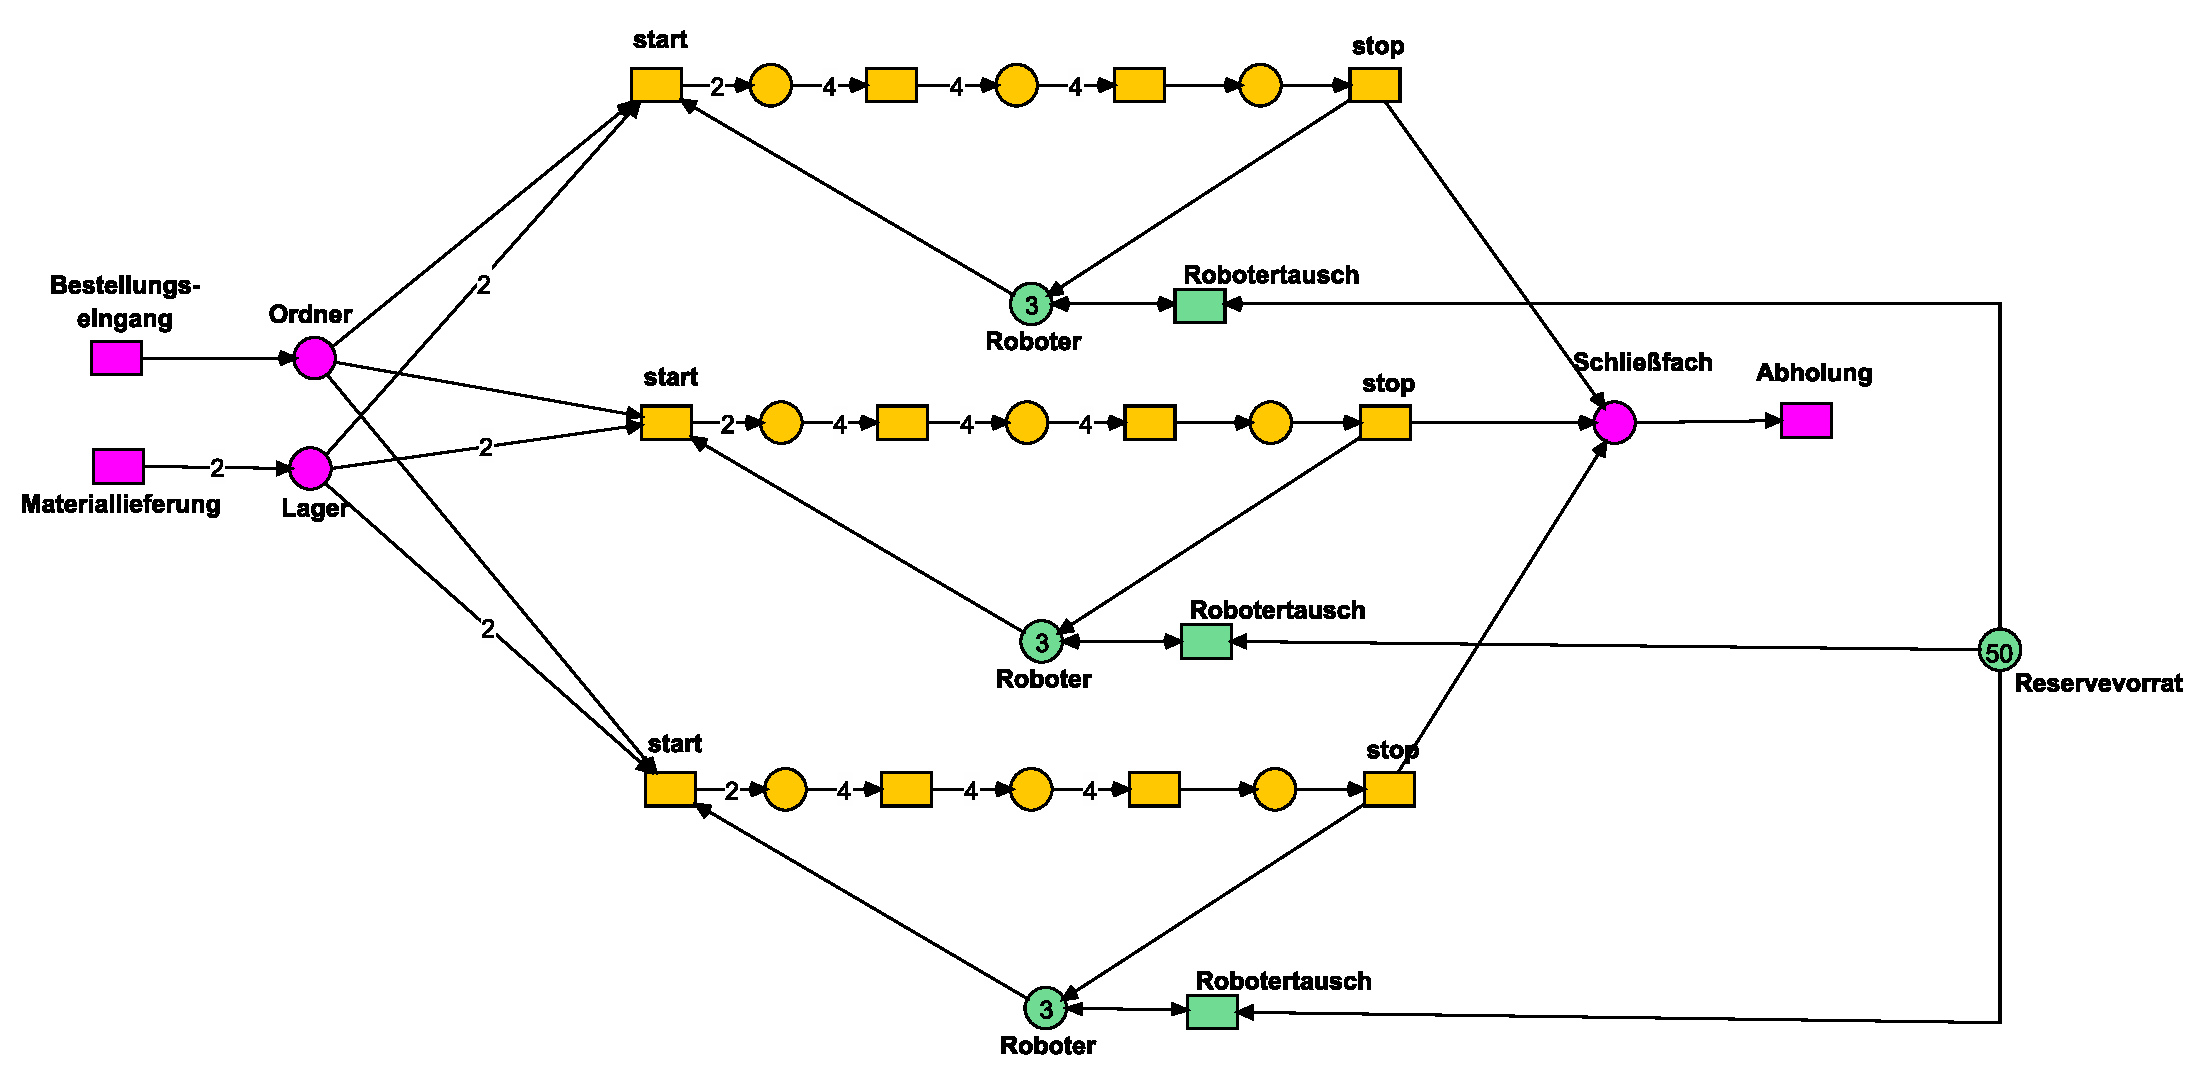
\includegraphics[scale=0.45]{aufgabe-8-6/8-6-4-roboter-reservevorrat.pdf}
}

Modell mit sychronen Kanälen:

\centerline{
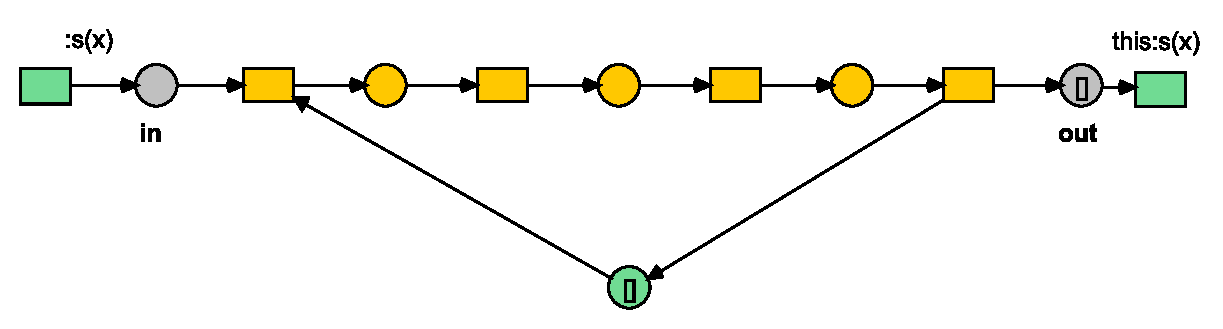
\includegraphics[scale=0.50]{aufgabe-8-6/8-6-5-synchrone-kanaele.pdf}
}


Schaltfolge, die zur Verklemmung von Maschine B führt: \(t_1 \cdot t_2 \cdot t_5\)

Es kommt zur Verklemmung, da beide Arbeitsbänder ihren Arbeitsprozess starten, aber nicht beenden können, falls das Werkzeug für den nächsten Schritt schon benutzt wird. Durch Hinzufügen eines Werkzeugs in \(p_{10}\) löst man dieses Problem, da nun in jeder erreichbaren Markierung mindestens ein Arbeitsband weiter schalten kann.

\end{document}